\documentclass[twoside]{article}

\usepackage{aistats2027}
%\usepackage[accepted]{aistats2027}
%\usepackage[preprint]{aistats2027}
\usepackage{amsmath,amssymb}
\usepackage{booktabs}
\usepackage{graphicx}
\usepackage{xcolor}
\usepackage[round]{natbib}
\renewcommand{\bibname}{References}
\renewcommand{\bibsection}{\subsubsection*{\bibname}}

% FLOATS. Figures are drawn at the width they print at (paper/scripts/common.py: 6.75in = \textwidth for
% figure*, 3.25in = \columnwidth for figure), so their text keeps its size. Let floats share a page with
% text before LaTeX sends them to a page of their own.
\renewcommand{\topfraction}{0.9}
\renewcommand{\dbltopfraction}{0.9}
\renewcommand{\bottomfraction}{0.5}
\renewcommand{\textfraction}{0.1}
\renewcommand{\floatpagefraction}{0.8}
\renewcommand{\dblfloatpagefraction}{0.8}
\setcounter{topnumber}{3}
\setcounter{dbltopnumber}{2}
\setcounter{totalnumber}{4}

% MARKERS
\newcommand{\TBD}[1]{\textcolor{red}{[TBD\ifx\relax#1\relax\else: #1\fi]}}
\newcommand{\NI}[1]{\textcolor{red}{[TBD: #1]}}
\newcommand{\review}[1]{\textcolor{blue}{#1}}
\newcommand{\new}[1]{\textcolor{green!45!black}{#1}}   % inserted/corrected in the results pass
\newcommand{\src}[1]{{\footnotesize\texttt{#1}}}
\newcommand{\nb}{\bar n}
\newcommand{\pc}{\mathbf{x}}
\newcommand{\rc}{\mathbf{y}}
\newcommand{\kpar}{\kappa}
\newcommand{\mo}{\mu}

\begin{document}

\twocolumn[
\aistatstitle{Inferring Spatial Point Processes from a Single Realization with Topological Deep Learning}
\aistatsauthor{Anonymous Author(s)}
\aistatsaddress{Anonymous Institution(s)} ]

%==============================================================================

\begin{abstract}
Spatial point processes (SPPs) are widely used to model data consisting of discrete event locations. A range of statistical
models has been developed to capture spatial interactions, from homogeneous Poisson processes describing complete spatial
independence to models capturing clustering, repulsion, and more complex spatial dependence. In many applications,
only a single point pattern is available, and we seek a plausible generative model from which additional patterns with a
similar underlying distribution can be simulated. This requires selecting an appropriate model family and estimating its parameters
from a single realization. We develop a unified pipeline for these tasks across multiple SPP families,
in which neural networks trained on simulated patterns combine classical spatial summary statistics with
topological features derived from persistent homology. We show that these features improve estimation performance,
with the resulting pipeline achieving state-of-the-art results on classical benchmarks.
In addition, we analyze the state space of the classification problem, characterizing regimes in which different point process
families are indistinguishable. Nevertheless, we show that even in these ambiguous regimes, our pipeline can generate new
realizations that preserve the statistical properties of the observed pattern.
Together, these results provide a practical framework for fitting spatial models and simulating patterns
consistent with the observed data.
\end{abstract}

%==============================================================================

\section{INTRODUCTION}
\label{sec:intro}

\begin{itemize}
  \item Setting: a single observed pattern; we want a plausible generative model from an established parametric
        family, from which similar patterns can be simulated. This means selecting the family and estimating its
        parameters from one realization.
  \item Hook: classification accuracy over the 8 families looks weak ($0.45$; $0.75$ in the structured regime), yet the
        end-to-end skill of the fitted models is high ($0.90$, against $0.74$ for minimum contrast, whose gap comes
        from the two families $K$ cannot fit). Classification errors cost no fidelity: skill $0.90$ with the
        predicted family vs $0.89$ with the correct one.
  \item Why accuracy is the wrong target near CSR: every model struggles on patterns near complete spatial randomness,
        and any prior that is not cherry-picked produces many of them. This is a property of the problem, not a
        failure of the models. What matters is whether the fitted model reproduces the pattern.
  \item Contributions:
  \begin{enumerate}
    \item \textbf{Scoring} (Section~\ref{sec:score}): a fit is scored by how well its simulations match an independent held-out
          replicate, with a strictly proper kernel score on local configurations, reported as skill between CSR
          and the true model.
    \item \textbf{Regime boundary} (Section~\ref{sec:analysis}): for every family except cell, detectability from CSR is governed by one
          physical coordinate (cluster overlap $\omega$ or a pair-count signal-to-noise ratio $\zeta$) times a fitted
          power of $\nb$. Before this boundary even the oracle does not beat Poisson.
    \item \textbf{Pipeline} (Sections~\ref{sec:model} and~\ref{sec:analysis}): classifier then family-specific estimator,
          $p(f,\theta\mid x)=p(f\mid x)\,p(\theta\mid x,f)$. Structured patterns sent to Poisson cost nothing,
          wrong-family fits are about as good as right-family ones. The pipeline beats minimum contrast at
          selection; end to end, it matches minimum contrast given the true family where $K$ can be fitted, and
          fits Strauss and cell, where it cannot.
    \item \textbf{TDA features} (Section~\ref{sec:analysis}): in the structured regime, persistent homology cuts
          estimation error by $26\%$ on Strauss and $18\%$ on cell, the two families minimum contrast cannot fit
          (cell has $K(r)=\pi r^2$ exactly); alpha carries Strauss and DTM$_{10}$ cell.
  \end{enumerate}
\end{itemize}

%==============================================================================

\section{BACKGROUND}
\label{sec:setting}
\label{sec:spp}

We define notation, review the summary statistics that serve as ParamNet's classical features, and introduce the eight families we consider.
A spatial point process $X$ is a random collection of points in $\mathbb{R}^n$. We focus on single realizations of $X$ restricted to $W \subseteq \mathbb{R}^2$, i.e. $\pc = X \cap W$. We write $\pc := \{x_1, \dots, x_{N(W)}\}$, where the number of points $N(W)$ is random with $\mathbb{E}N(W) = \nb$.

\paragraph{Summary statistics.}
Second-order and nearest-neighbor summary statistics are widely used to analyze SPPs. We consider the $K$, $L$, $F$, $G$, and $J$ functions defined for a stationary process with intensity $\lambda$. Ripley's $K$
function is defined so that $\lambda K(r)$ is the expected number of further points within distance $r$ of a typical
point in $X$. The $L$ function,
\[
  L(r)=\sqrt{K(r)/\pi},
\]
rescales $K$ to units of distance, and is more widely used in practice. For small $r$, $L(r) - r > 0$ can suggest clustering, and  $L(r) - r < 0$ suggests regularity.

The remaining functions are based on distances to the nearest point of $X$. The empty-space function
\[
  F(r)=\mathbb{P}\bigl(d(u,X)\le r\bigr)
\]
is the distribution of the distance from an arbitrary fixed location
$u\in\mathbb{R}^2$ to the nearest point of $X$. The nearest-neighbor function
\[
  G(r)=\mathbb{P}\bigl(d(x,X\setminus\{x\})\le r\bigr)
\]
is the distribution of the distance from a typical point $x$ of
$X$ to its nearest neighbour. Intuitively, $F$ measures the size of the gaps between points, while $G$ measures how
tightly points are packed around each other. The $J$ function combines them,
\[
  J(r)=\frac{1-G(r)}{1-F(r)}, \qquad F(r)<1,
\]
and compares what a typical point sees with what an arbitrary location sees: $J(r)<1$ indicates that points are closer
to each other than arbitrary locations are to points (clustering), and $J(r)>1$ indicates the opposite (regularity).

\paragraph{Families.}
\label{sec:families}
We consider eight families of stationary SPPs (Table~\ref{tab:families}, Figure~\ref{fig:examples}; definitions in Appendix~\ref{app:families}). The homogeneous Poisson process serves as the model for \emph{complete spatial randomness} (CSR). We include four \emph{clustered} families: three Neyman--Scott processes, in which Poisson parents generate offspring displaced by a kernel (Thomas, nested Thomas, and ring), and the log-Gaussian Cox process (LGCP), whose intensity is a random field. Additionally, we consider two \emph{regular} families: Mat\'ern~II, which thins a Poisson process to enforce a hard-core distance $R$, and Strauss, which penalizes (rather than forbids) pairs closer than $R$. Finally, the Baddeley--Silverman cell process has $K(r)=\pi r^2$ exactly, so it is indistinguishable from CSR at second order despite not being Poisson; this motivates the use of topological features (Section~\ref{sec:inputs}).

Every family except cell approaches CSR along a single regime coordinate (Table~\ref{tab:families}; Section~\ref{sec:analysis}): for the Neyman--Scott families the cluster overlap $\omega=\sigma\sqrt\kappa$ represents the cluster scale in units of the parent spacing. We obtain crisp clusters for $\omega\ll1$ and approach CSR as $\omega\to\infty$. Furthermore, some non-Poisson families approach one another over part of their respective parameter spaces. \review{Notably, Thomas, nested and ring (Appendix~\ref{app:families-limits}).}

\begin{table}[t]
\caption{The eight families, grouped by second-order structure, with their parameters and the regime coordinate
$\eta$ that governs detectability (Section~\ref{sec:analysis}). $\omega$: cluster overlap, the cluster scale
in units of the parent spacing ($\omega_{\rm in}$: of the inner level of nested); $\zeta$: a pair-count
signal-to-noise ratio, for the regular families the expected number of missing close pairs. Patterns approach CSR
as $\omega$ grows or $\zeta$ shrinks. Every family except cell has one such coordinate; cell matches CSR at second
order.}
\label{tab:families}
\begin{center}
\footnotesize
\setlength{\tabcolsep}{4pt}
\begin{tabular}{@{}lll@{}}
\toprule
Family & Parameters & Regime coordinate \\
\midrule
Poisson (CSR) & $\nb$ & --- \\
\addlinespace[2pt]
\multicolumn{3}{@{}l}{\emph{Clustered}} \\
Thomas       & $\kappa,\mu,\sigma$ & $\omega=\sigma\sqrt\kappa$ \\
Nested       & $\kappa,\mu_1,\mu_2,\sigma_1,\sigma_2$ & $\omega_{\rm in}=\sigma_2\sqrt{\kappa\mu_1}$ \\
Ring         & $\kappa,\mu,\rho,\sigma$ & $\omega=\rho\sqrt\kappa$ \\
LGCP         & $\mu_{\log},\sigma^2,s$ & $\zeta=(e^{\sigma^2}-1)\,s\,\nb$ \\
\addlinespace[2pt]
\multicolumn{3}{@{}l}{\emph{Regular}} \\
Mat\'ern II  & $R,\lambda_p$ & $\zeta=R\,\nb$ \\
Strauss      & $\nb,q,R$ & $\zeta=q\,R\,\nb$ \\
\addlinespace[2pt]
\multicolumn{3}{@{}l}{\emph{Second-order CSR}} \\
Cell         & $\nb,k$ & none (U-shaped in $k$) \\
\bottomrule
\end{tabular}
\end{center}
\end{table}

\begin{figure*}[t]
\centering
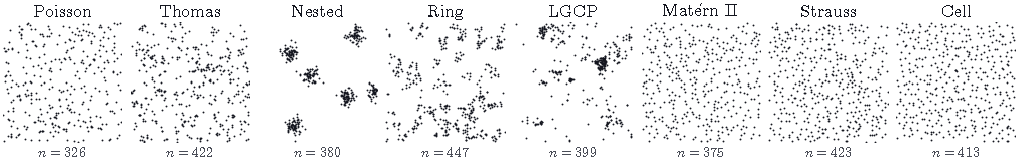
\includegraphics[width=\textwidth]{figs/v2/f1_examples}
\caption{Example realizations on $W=[0,1]^2$ of the eight families in structured regimes. $n$: number of points.}
\label{fig:examples}
\end{figure*}


%==============================================================================

\section{DATA GENERATION}
\label{sec:data}

We train and evaluate on synthetic patterns, simulated with standard algorithms, so that the true family and parameters are known. For each family $f$ we construct a prior $\pi_f$ over its parameter space. We then draw parameters $\theta\sim\pi_f$ and simulate two independent replicates on $W = [0, 1]^2$ for each $(f, \theta)$. The first realization, $\pc_{f, \theta}$, acts as the observed pattern and is the input to the pipeline. The second realization, $\rc_{f, \theta}$, is held out and used to score a model's fit (Section~\ref{sec:score}).

\paragraph{Priors.} Each $\theta$ is drawn in three steps. First, the expected number of points in $W$ is drawn as $\nb\sim\text{log-uniform}[50,950]$, this is the same for every family. Second, the remaining degrees of freedom are drawn log-uniformly in scale-free units, for example the overlap $\omega$ for the cluster families and $R\sqrt{\nb}$ for the hard-core families. Each range extends from strongly structured patterns to pattern indistinguishable from CSR. Finally, the last parameter is solved so that  $\mathbb{E}\,N(W)=\nb$ (e.g.\ $\kappa=\nb/\mu$ for Thomas). The only draws excluded are degenerate cluster patterns, with fewer than four effective clusters in $W$. \review{We deliberately keep our priors as wide and un-curated as possible to reflect ...} Ranges and simulator setting as in Appendix~\ref{app:data}.

\paragraph{Size and splits.}
\review{For each family, we draw $50\,000$ parameter vectors with two replicates each, $100\,000$ patterns per family and $800\,000$ in total.} The data is split by $\theta$ into train, test, and validation blocks of $37\,000$, $12\,000$, and $1\,000$ parameter vectors, respectively. \review{Both replicates of each $\theta$ fall in the same block, so no parameter setting seen in training appears in the test block.} See Appendix~\ref{app:data} for details on sweep ranges, constraints and simulator settings.

%==============================================================================

\section{PARAMNET}
\label{sec:model}

Given an input pattern $\pc_{f, \theta}$, our pipeline produces a fit $\hat P = (\hat f, \hat\theta)$ via a two-step procedure,
\[
  p(f,\theta\mid \pc_{f, \theta})=p(f\mid \pc_{f, \theta})\,p(\theta\mid \pc_{f, \theta},f).
\]
An 8-way classifier predicts $\hat f$, followed by a family-specific estimator that produces $\hat\theta$. In place of a learned estimator, patterns classified as Poisson automatically receive $\hat \lambda=n$, which is the exact maximum-likelihood estimate.

Both stages of \emph{ParamNet} share a single architecture, trained once as the classifier and once (per family) as an estimator (Figure~\ref{fig:pipeline}). ParamNet receives two descriptions of $\pc_{f, \theta}$: classical features derived from second-order summaries, and topological features obtained by vectorizing persistence diagrams. Each feature type passes through its own convolutional encoder, and the resulting embeddings are concatenated with $\log n$ before a shared FCNN head.

\begin{figure*}[t]
\centering
\framebox[\textwidth]{\rule{0pt}{1.6in}\TBD{pipeline figure}}
\caption[Pipeline]{\TBD{pipeline figure, one row: pattern $\to$ summary curves and persistence images $\to$ encoders $\to$
head $\to(\hat f,\hat\theta)\to$ simulations $\to$ kernel score against $y_{f,\theta}$, with $P^0$ and
$P^\star$ as references.}}
\label{fig:pipeline}
\end{figure*}

\paragraph{Classical features.}
\label{sec:inputs}
Let $\alpha(r)$ be a second-order summary function in $\{L(r)-r, F(r), G(r), J(r)\}$. We compute each of these functions at $512$ linearly-spaced radii in the interval $(0, 0.25]$. For each function, we obtain a feature vector $[\alpha(r_1), \dots, \alpha(r_{512})] \in \mathbb{R}^{512}$. \review{For $L$ we apply Ripley's isotropic edge correction; for $F$ and $G$ we apply the border (reduced-sample) correction, which $J=(1-G)/(1-F)$ inherits.} The four vectors are stacked as channels of a single tensor of shape $(N, 4, 512)$, where each channel is $z$-scored using train-set mean and standard deviation.

\paragraph{Topological features.}
We compute the $H_0$ and $H_1$ persistence diagrams using two complementary filtrations, alpha and DTM$_{10}$, obtaining four diagrams per pattern. \review{In Section~\ref{sec:analysis} we show that both are needed, and neither suffices individually.} Each persistence diagram is vectorized into a \emph{persistence image}. The four persistence images are encoded separately: \review{a $64\times64$ image for alpha-$H_1$, DTM$_{10}$-$H_0$ and DTM$_{10}$-$H_1$, and a $64$-dimensional vector for alpha-$H_0$, whose births are identically zero.} See Appendix~\ref{app:features} for a full treatment of the vectorization process and its hyperparameters.

\paragraph{Classical encoders.}
\label{sec:architecture}
The classical feature's $(N,4,512)$ tensor passes through a 1-D convolutional encoder: three blocks of kernel-$3$, padding-$1$ convolutions with channel widths $32\to64\to128$, each followed by ReLU; between blocks, average pooling (kernel $2$) and channel-wise dropout ($p=0.2$) downsample and regularize. Rather than pooling the final feature map to a single value per channel, we apply an adaptive average pool to a fixed width of $4$. Position along $r$ is part of the signal so, being translation-invariant, a global average would leave the encoder unable to distinguish \review{a feature at small $r$ from the same feature at large $r$.} The resulting $128\times4$ map is flattened and passed through a linear layer with ReLU to produce a $64$-dimensional embedding.

\paragraph{Topological encoders.}
The four persistence images are encoded independently by their own copy of the same conv-pool-dropout architecture (channels $32\to64\to128$, kernel $3$, dropout $0.2$, adaptive pool to width $4$). We use 2-D for the three images and 1-D for alpha-$H_0$. Encoders are not shared across filtration or homology dimension because the persistence image axes are calibrated per-(filtration, dimension) pair, so the same pixel coordinate means something different in each. The independent encoders produce four $64$-dimensional embeddings.

\paragraph{FCNN head.}
The classical and topological embeddings are concatenated with standardized $\log n$, giving a $321$-dimensional input to the shared head. Two fully-connected layers ($64$, $32$) with ReLU and dropout ($p=0.1$) are followed by a final linear layer \review{with either $8$ logits (classification) or a scalar output for each family parameter (inference).}

%==============================================================================

\section{TRAINING PROCEDURE}
\label{sec:training}

We describe how ParamNet, and the models with which it is compared, are trained and evaluated. We evaluate the overall fidelity of the end-to-end pipeline, as well as the individual components of the pipeline independently.

\paragraph{Training.}
Every network is trained using the same \review{recipe}: AdamW with learning rate $10^{-3}$, batch size $128$, \review{at most $200$
epochs,} early stopping on validation loss with patience $30$, and the best-validation weights restored. The
classifier minimizes class-weighted cross-entropy, while the parameter estimators minimize squared error on standardized $\log\theta$.
\review{Because the recipe is shared, a difference between two networks is a difference in their inputs.} Settings, parameter
counts and training cost are in Appendix~\ref{app:models}.

\paragraph{Controls.}
\label{sec:learners}
As controls we train gradient-boosted trees on feature tables of the summary curves, of persistence summaries, and of
both, and a logistic regression on the summary curves. We also retrain ParamNet with the persistence images removed,
or with one filtration only, and nothing else changed (Appendix~\ref{app:models}).

\paragraph{Classical baseline.} Our classical baseline is minimum contrast on $K$, with penalized-contrast model
selection among Poisson and the families that have a closed-form $K$. Strauss and cell have none, so it can neither
select nor fit them; given either, it falls back to the training median. We also run it given the true family, which
removes its selection errors.

\paragraph{Evaluation.} Every model is scored on the same held-out test patterns. For classification we report
balanced accuracy over the eight families, and over the four mechanisms (CSR, clustered, regular, cell). For
inference, we report the estimator error $\mathrm{RMSE}(\log\theta)/\mathrm{s.d.}$ averaged over a family's targets,
where $1$ is the error of predicting the training mean.


\subsection{Goodness of Fit}
\label{sec:score}

Accuracy and estimation error in terms of RMSE on log-normalized parameters does not tell us whether the fitted model reproduces the observed pattern, nor does it provide clear intuition of the model's performance. We therefore score the test set on fidelity directly.

Let $\{\pc_{f_1, \theta_1}, \dots \pc_{f_N, \theta_N}\}$ be the test patterns, with held-out replicates $\{\rc_{f_1, \theta_1}, \dots \rc_{f_N, \theta_N}\}$. For test pattern $\pc_{f_i, \theta_i}$ with ParamNet fit $\hat P_i=(\hat f_i,\hat\theta_i)$, write $P^\star_i=(f_i,\theta_i)$ for the oracle and $P^0_i = (\text{Poisson}, \hat \lambda)$ for the CSR fit. Each $P_i\in\{\hat P_i,P^\star_i,P^0_i\}$ is scored by comparing the held-out replicate $\rc_{f_i, \theta_i}$ to $16$ independent simulations $z_1,\dots,z_{16}\stackrel{\text{iid}}\sim P_i$ on $W$, using a kernel score on local configurations. Its properties and validation are in Appendix~\ref{app:score}.

\paragraph{Local configurations.}
For a pattern $z$ with $n$ points, rescale to unit intensity, $\tilde z=\sqrt n\,z$, and fix a centre set $C(z)\subseteq\tilde z$ of size $m=\min(n,300)$, drawn uniformly at random. Each centre $p\in C(z)$ gives a local configuration
\begin{align}
    N_R(p,\tilde z) &= \{q\in\tilde z\setminus\{p\}:\|q-p\|\le R\}, \\
    \phi(p;z) &= \frac1R\big(N_R(p,\tilde z)-p\big),
\end{align}
with $R=1.5$ (in units of mean spacings since $\tilde z$ has unit intensity). We write $\phi_1,\dots,\phi_m$ for the local configurations of the held out $\rc_{f_i, \theta_i}$.

\paragraph{Kernel score.}
Local configurations are compared by an RBF kernel between Gaussian-smoothed occupancy measures on a $21\times21$ grid,
\begin{align}
    \mu_\phi(u) &= \sum_{p\in\phi}e^{-\frac{|u-p|^2}{2h^2}},\\
    k(\phi,\psi) &= e^{-\frac{\|\mu_\phi-\mu_\psi\|^2}{2\ell^2}},
\end{align}
with $h=0.1$ and bandwidth $\ell$ fixed to the median pairwise distance among $\mu_{\phi_1},\dots,\mu_{\phi_m}$ \review{(before any model is scored).}

A model $P_i$ is scored against $\rc_{f_i, \theta_i}$ by the kernel score
\begin{equation}
  S(P_i,\rc_{f_i, \theta_i})=\tfrac12\,\mathbb{E}\,k(\Phi,\Phi')-\frac1m\sum_{i=1}^{m}\mathbb{E}\,k(\phi_i,\Phi),
  \label{eq:kernel}
\end{equation}
where $\Phi,\Phi'$ are local configurations $\phi(p;z_k),\phi(p';z_{k'})$ at centres drawn from two \emph{different} simulations $z_k,z_{k'}$ ($k\ne k'$) of $P_i$, with expectations estimated by averaging over the $16$ simulations above.

\paragraph{Skill.}
For test set $\{\pc_{f_1, \theta_1}, \dots \pc_{f_N, \theta_N}\}$, skill sums (over $i=1,\dots,N$) how each fit's kernel score on $y_{f_i, \theta_i}$ compares to $P^0_i$ and $P^\star_i$ (reported only when the denominator is resolved).
\begin{equation}
  \mathrm{skill}=\frac{\sum_i\big[S(P^0_i,y_{f_i, \theta_i})-S(\hat P_i,y_{f_i, \theta_i})\big]}{\sum_i\big[S(P^0_i,y_{f_i, \theta_i})-S(P^\star_i,y_{f_i, \theta_i})\big]}
  \label{eq:skill}
\end{equation}
Skill $0$ means no better than CSR and skill $1$ as good as the truth; on a finite set of patterns a fit can score
slightly above $1$. A fit's \emph{gain over CSR} on pattern $i$ is $S(P^0_i,y_i)-S(P,y_i)$, the amount by which it
improves on the CSR reference; skill weights each pattern by the true model's gain, so patterns on which no model
beats CSR carry no weight.

\paragraph{Evaluation set.}
We score fits on $1\,440$ test patterns: $60$ per regime stratum (below the boundary at $\tau=0.5$, between $\tau=0.5$
and $0.9$, and beyond $\tau=0.9$; Section~\ref{sec:analysis}) for each family with a coordinate, $60$ per band of $k$
for cell ($k=2$, $3$--$4$, $\ge5$), and $180$ Poisson patterns ($1\,439$ scored: one ring pattern's gain could not be
resolved). Intervals are $95\%$ bootstrap intervals over patterns, and every difference is paired: same patterns, same
simulations.

%==============================================================================

\section{EXPERIMENTS ON SIMULATED PATTERNS}
\label{sec:analysis}

We score ParamNet end-to-end on the $1\,440$ patterns of the evaluation set, and its classifier on all
$192\,000$ test patterns (Section~\ref{sec:score}). We find that ParamNet's fits reproduce held-out data nearly as well as the true model, and better than minimum contrast. The modest classification accuracy is set by the data, not by the model. Moreover, ParamNet's classification errors cost almost no fidelity.

\begin{table*}[t]
\caption{Main results. \emph{Identification}: balanced accuracy over the eight families on the $192\,000$ test
patterns, on all of them and in the structured regime ($\tau{=}0.9$), and over the four mechanisms (CSR, clustered,
regular, cell) at $\tau{=}0.9$; intervals are within $\pm0.003$. Minimum contrast never selects Strauss or cell.
\emph{Fidelity}: skill on the $1\,439$ scored patterns ($1$: as good as the true model; $0$: no better than CSR), given
the predicted family, given the true family, and on the non-Poisson patterns routed to a wrong family. $\Delta$:
ParamNet $-$ minimum contrast, paired, overall and by whether minimum contrast can fit the family. Intervals are $95\%$
bootstrap over patterns; higher is better. Accuracy is modest, yet the fits recover $90\%$ of the true model's gain.}
\label{tab:main}
\begin{center}
\footnotesize
\setlength{\tabcolsep}{4pt}
% generated by paper/scripts -- do not edit; rerun python paper/scripts/make.py
\begin{tabular}{@{}lrrrrrr@{}}
\toprule
 & \multicolumn{3}{c}{Identification (balanced accuracy)} & \multicolumn{3}{c}{Fidelity (skill)} \\
\cmidrule(lr){2-4} \cmidrule(lr){5-7}
 & All & $\tau{=}0.9$ & Mechanism & Predicted family & True family & Wrong family ($n$) \\
\midrule
ParamNet & 0.450 & 0.754 & 0.899 & $0.90$ {\scriptsize[$0.85$, $0.95$]} & $0.89$ {\scriptsize[$0.84$, $0.94$]} & $0.82$ {\scriptsize[$0.73$, $0.90$]} ($350$) \\
Minimum contrast & 0.255 & 0.408 & 0.633 & $0.74$ {\scriptsize[$0.65$, $0.81$]} & $0.78$ {\scriptsize[$0.65$, $0.87$]} & $0.57$ {\scriptsize[$0.40$, $0.70$]} ($647$) \\
\midrule
$\Delta$, all families &  &  &  & $+0.16$ {\scriptsize[$+0.08$, $+0.26$]} & $+0.11$ {\scriptsize[$+0.04$, $+0.21$]} &  \\
$\Delta$, closed-form $K$ &  &  &  & $+0.06$ {\scriptsize[$-0.00$, $+0.15$]} & $+0.04$ {\scriptsize[$-0.03$, $+0.14$]} &  \\
$\Delta$, Strauss, Cell &  &  &  & $+1.27$ {\scriptsize[$+0.71$, $+2.04$]} & $+0.97$ {\scriptsize[$+0.80$, $+1.17$]} &  \\
\bottomrule
\end{tabular}

\end{center}
\end{table*}

\paragraph{High fidelity fits.}
ParamNet reaches skill $0.90$ [$0.85$, $0.95$]: its fits recover $90\%$ of what the true model gains over CSR.
By comparison, minimum contrast reaches $0.74$ [$0.65$, $0.81$] on the same patterns, \review{a paired gap of $+0.16$ [$+0.08$, $+0.26$], and $+0.11$ [$+0.04$, $+0.21$] when both are given the true family.} ParamNet's advantage is concentrated in the Strauss and cell families, which have no closed-form $K$. On these two families ParamNet reaches skill $0.93$ [$0.79$, $1.06$], while minimum contrast, even when given the true family, does no better than CSR ($-0.04$ [$-0.17$, $+0.08$]; per family:
Table~\ref{tab:families-skill}). 


ParamNet's advantage is also visible in the estimators' loss: given the true family, every learned estimator has lower $\mathrm{RMSE}(\log\theta)/\mathrm{s.d.}$ than minimum contrast on every family. On the Neyman--Scott families minimum contrast does worse than predicting the training mean ($1.48$- $2.25$; Appendix~\ref{app:estimation}).

\begin{figure*}[t]
\centering
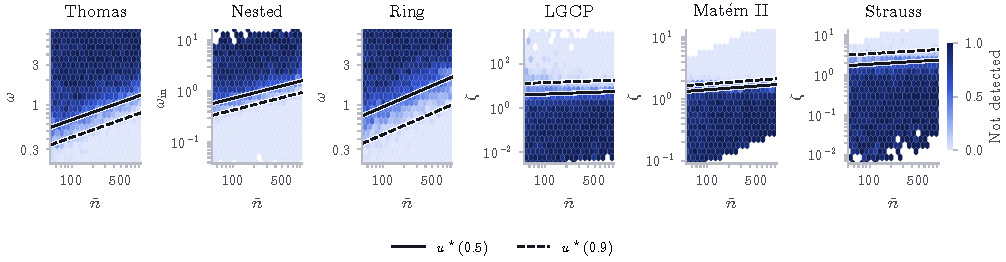
\includegraphics[width=\textwidth]{figs/v2/s_regime_map}
\caption{The regime boundary in the physical parameters: share of test patterns the reference detector (trees on the
summary curves, size $5\%$) does not detect, over $\nb$ and each family's regime coordinate $\eta$
(Table~\ref{tab:families}). Each boundary is a line $u=\log\eta+a\log\nb=u^\star(\tau)$: $\tau=0.5$ solid, $0.9$
dashed. Patterns approach CSR as $\omega$ grows or $\zeta$ shrinks.}
\label{fig:regime-map}
\end{figure*}

\paragraph{Classification difficulty is inherent.}
The deliberately wide priors admit many near-CSR patterns, on which every method struggles to identify the family.
We call a pattern \emph{detectable} if a test of CSR rejects it. Every test we use is calibrated to falsely reject
only $5\%$ of truly Poisson patterns, so rejection is real evidence of structure. For each family, the share of
patterns detected is governed by one physical coordinate (Table~\ref{tab:families}), so the undetectable region is
bounded by a single curve in parameter space (Figure~\ref{fig:regime-map}). The \emph{$\tau$-boundary} is the curve along which a fraction $\tau$
of a family's patterns are detected; patterns beyond it are detected more often. We fit it on a reference detector,
trees on the summary curves (Appendix~\ref{app:regime}). Detectability is a property of the patterns, not of the test.
The $L$ test, trees on persistence summaries alone and ParamNet, thresholded to the same false-positive rate, detect
the same share of every family's patterns to within three points, and meet the same boundary
(Figure~\ref{fig:regime}; Table~\ref{tab:regime}). Restricting to patterns beyond the $\tau=0.5$ boundary raises
ParamNet's accuracy from $0.45$ to $0.70$, and beyond $\tau=0.9$ to $0.75$ (per learner:
Table~\ref{tab:classification}). Below the $\tau=0.5$ boundary ParamNet
calls $61\%$ of patterns Poisson, and even the true model gains nothing over CSR (Figure~\ref{fig:regime-detect}).


\begin{figure}[t]
\centering
% Panel (a) of f4_regime, cropped; f4_regime.py now also writes it alone as f4_detection.pdf.
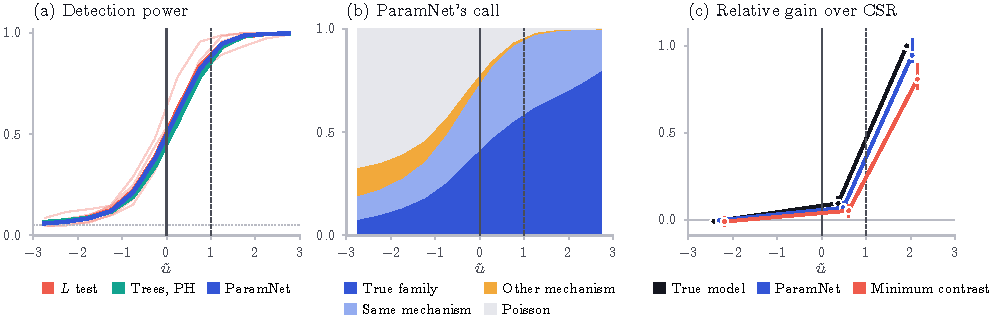
\includegraphics[width=0.8\columnwidth,trim=0 0 331 11,clip]{figs/v2/f4_regime}
\caption{Detection power of three tests of size $5\%$ (dotted) against the rescaled regime coordinate $\tilde u$
(Figure~\ref{fig:regime-detect}),
families averaged; faint: the $L$ test per family. Solid: the $\tau=0.5$ boundary; dashed: $\tau=0.9$. The
boundaries are fitted on a fourth detector, so the agreement is not by construction.}
\label{fig:regime}
\end{figure}

\paragraph{Errors cost almost no fidelity.}
ParamNet makes two kinds of error, and we show that neither result in significant loss of fidelity. Supplying ParamNet with the true family changes its skill by $-0.01$ [$-0.03$, $+0.02$], implying that patterns that get misclassified in the end-to-end pipeline still receive a high-fidelity fit. In fact, wrong-family fits keep $82\%$ of the true model's gain (against $91\%$ when the family is identified), because the confusions occur between look-alikes: in the structured regime $96\%$ stay within one mechanism (clustered, regular, cell; Figure~\ref{fig:confusion}), and three quarters are among Thomas, nested and ring, which produce the same patterns over part of their parameter spaces (Appendix~\ref{app:families-limits}). Calling a pattern Poisson costs nothing: on the $271$ patterns ParamNet sends to Poisson, the true model does no better than CSR, and the $L$ test rejects CSR on only $2.2\%$ [$1.0$, $4.7$] of them, no more often than on Poisson patterns. For these patterns, CSR is essentially the correct fit.

\paragraph{Topology helps where minimum contrast cannot fit.}
To investigate the value of each filtration, we retrain ParamNet on alpha alone and on DTM$_{10}$ alone.
Table~\ref{tab:topology} shows that the two are complementary. Alpha alone cuts estimation error on Strauss by
$28\%$, as much as both filtrations together ($26\%$), while DTM$_{10}$ alone does the same for cell ($19\%$ against
$18\%$). Neither does both: alpha gets only $11\%$ on cell and DTM$_{10}$ only $10\%$ on Strauss, which is why
ParamNet uses both. Together, the persistence images cut error by $26\%$ on Strauss and $18\%$ on cell, the two
families that minimum contrast cannot fit.

\paragraph{Summary.}
(i) ParamNet's fits reach skill $0.90$, against $0.74$ for minimum contrast; (ii) the data, not the model, limits accuracy: every detector meets the same boundary, and below it even the true model gains nothing over CSR; (iii) errors are cheap: supplying the true family changes skill by $-0.01$, and calling near-CSR patterns Poisson costs nothing; (iv) topology helps where minimum contrast fails, cutting estimation error on Strauss and cell by $26\%$ and $18\%$.

\begin{table}[!htb]
\caption{Relative change in estimation error $\mathrm{RMSE}(\log\theta)/\mathrm{s.d.}$ ($\tau{=}0.9$) when persistence
images are added to the same network on the summary curves (``Curves alone'': its error). Negative is better; one
training seed (intervals: Appendix~\ref{app:filtrations}). The images help where minimum contrast cannot fit.}
\label{tab:topology}
\begin{center}
\footnotesize
% generated by paper/scripts -- do not edit; rerun python paper/scripts/make.py
\begin{tabular}{@{}lrrrr@{}}
\toprule
 & Curves alone & + both & + alpha & + DTM \\
\midrule
Strauss & 0.152 & $-$26\% & $-$28\% & $-$10\% \\
Cell & 0.173 & $-$18\% & $-$11\% & $-$19\% \\
\midrule
Thomas & 0.415 & $-$2\% & +3\% & +3\% \\
Nested & 0.576 & $-$1\% & $-$1\% & $-$1\% \\
Ring & 0.457 & +1\% & $-$2\% & 0\% \\
LGCP & 0.301 & $-$4\% & $-$2\% & $-$2\% \\
Mat\'ern II & 0.084 & +7\% & +6\% & +41\% \\
\bottomrule
\end{tabular}

\end{center}
\end{table}

%==============================================================================

\clearpage
\appendix
\onecolumn
\aistatstitle{Supplementary Materials}

% Outline. The previous appendix text is in backup_pre_restructure/appendix_pre_outline.tex.
% Markers: (new) = not written anywhere yet; (moved) = text exists elsewhere; (blocked) = needs a run.

%==============================================================================
\section{FAMILIES}
\label{app:families}

\begin{itemize}
  \item Definitions, one paragraph each; trim the Poisson paragraph.
  \item Closed-form $K$ for the families that have one. (new; minimum contrast depends on them)
  \item Regime coordinates, one-line rationale each. (moved from Appendix~\ref{app:regime})
  \item \label{app:families-limits}Near-equivalences between families: ring $\to$ Thomas as $\rho/\sigma\to0$; nested $\to$ Thomas for large $\sigma_1$; Mat\'ern~II $\approx$ Strauss as $q\to1$.
\end{itemize}

%==============================================================================
\section{SIMULATION}
\label{app:data}

\begin{itemize}
  \item Prior table: family, sampled coordinates, ranges, solved parameter. Replaces the current bullets.
  \item Constraints: $\ge4$ effective clusters; conditioning on $n\in[20,2000]$ (range of the $L$ test's null tables; $304$ of $800\,304$ simulations redrawn); parent buffer.
  \item Simulators: Strauss MCMC (sweeps, convergence check), cell, Mat\'ern~II, LGCP field method and grid. (LGCP new)
  \item Volume; split by $\theta$.
  \item Cut the ``minimal curation'' bullets; one sentence in Section~\ref{sec:data} covers them.
\end{itemize}

%==============================================================================
\section{FEATURES}
\label{app:features}

\begin{itemize}
  \item Summary curves: estimators, edge corrections, $r$ grid, standardisation. (move the edge-correction sentence from Section~\ref{sec:model})
  \item Filtrations: alpha and DTM$_k$ definitions, $k=10$, software. (new; neither is defined anywhere)
  \item Persistence images: weighting, bandwidth, boxes, scaling by $\sqrt n$ and $n$, $\sqrt{\cdot}$ transform. (text in the backup; drop the Rips mention)
  \item Feature tables used by the trees. (new)
  \item Optional figure: mean persistence image per family (alpha-$H_1$, DTM-$H_0$).
\end{itemize}

%==============================================================================
\section{MODELS AND TRAINING}
\label{app:models}

\begin{itemize}
  \item Layer-by-layer architecture table. (move the encoder paragraphs from Section~\ref{sec:model}; saves about $0.25$ page)
  \item Training recipe, class weights, target standardisation. (text in the backup)
  \item Tree and logistic hyperparameters. (new)
  \item Parameter counts, hardware, wall clock (Table~\ref{tab:cost}); shorten the caption.
  \item Training-seed variation of the curves vs curves+PH comparison. (blocked: seedcheck)
\end{itemize}

\begin{table}[h]
\caption{Each model's input representation and training cost. ``Classifier'' is wall-clock seconds to train the one
$8$-way classifier until early stopping; ``Estimators'' is the same summed over the seven per-family estimators.
``Input'' names the tensors the model sees: \emph{curves} is the $(4,512)$ summary-function stack, \emph{classical}
the same curves as a feature table for the tree learners, and each filtration name a persistence summary of that
filtration's diagrams. \new{All four network rows} share one trainer and stopping rule, so their differences are the
cost of the persistence images alone. Lower is cheaper; cost is not the point of the comparison.}
\label{tab:cost}
\begin{center}
\footnotesize
% generated by paper/scripts -- do not edit; rerun python paper/scripts/make.py
\begin{tabular}{@{}lllrr@{}}
\toprule
Model & Learner & Input & Classifier (s) & Estimators (s) \\
\midrule
\texttt{fusion\_curves\_alpha\_dtm10} & nn & curves, alpha\_diameter,dtm\_k10 & 3,217 & 7,090 \\
\texttt{hgb\_classical} & hgb & classical & 414 & 132 \\
\texttt{hgb\_classical\_ph} & hgb & classical, ph\_alpha, ph\_dtm10 & 188 & 218 \\
\texttt{hgb\_ph} & hgb & ph\_alpha, ph\_dtm10 & 153 & --- \\
\texttt{linear\_classical} & linear & classical & 90 & --- \\
\texttt{nn\_curves} & nn & curves & 1,862 & 604 \\
\texttt{fusion\_curves\_alpha} & nn & curves, alpha\_diameter & 1,776 & 1,680 \\
\texttt{fusion\_curves\_dtm10} & nn & curves, dtm\_k10 & 2,081 & 1,744 \\
\bottomrule
\end{tabular}

\end{center}
\end{table}

%==============================================================================
\section{MINIMUM-CONTRAST BASELINE}
\label{app:mincontrast}

\begin{itemize}
  \item Contrast: $K$, $r$ range, exponents, optimizer, bounds, starting values. (new)
  \item Penalised selection: penalty, how it was tuned, on which split.
  \item Fallback to the training median for Strauss and cell; failure rate.
  \item Strauss has a standard maximum-pseudolikelihood fit: justify leaving it out, or add it as a baseline.
\end{itemize}

%==============================================================================
\section{KERNEL SCORE}
\label{app:score}

\begin{itemize}
  \item Propriety: state with a short proof (MMD identity), or drop ``Proposition'' and cite.
  \item Fixed choices: $R$, $h$, grid, $\ell$, $m$, edge rule, $16$ simulations.
  \item Skill estimator: ratio of sums, paired bootstrap, the ``resolved denominator'' rule, the one excluded ring pattern.
  \item Wrong-model ladder. (blocked: dose run on v2; v1 numbers cannot stay)
  \item Monte Carlo repeatability. (blocked: fidelity seeds 1--4)
\end{itemize}

%==============================================================================
\section{REGIME BOUNDARY}
\label{app:regime}

\begin{itemize}
  \item Detectors: $L$-test statistic and calibration; $5\%$ thresholds for the learned detectors; false-positive rates $0.045$--$0.053$.
  \item Fit of $a$ and $u^\star$; AUC of $u$ vs all parameters; agreement across detectors (Table~\ref{tab:regime}).
  \item Per-family detection and gain, cell against $k$ (Figure~\ref{fig:regime-detect}).
  \item Boundary in the physical parameters (Figure~\ref{fig:regime-map}).
  \item Gain over CSR per stratum and family. (moved from the old power subsection; now in Figure~\ref{fig:regime-detect})
  \item Construction of the evaluation strata.
\end{itemize}

\begin{figure}[t]
\centering
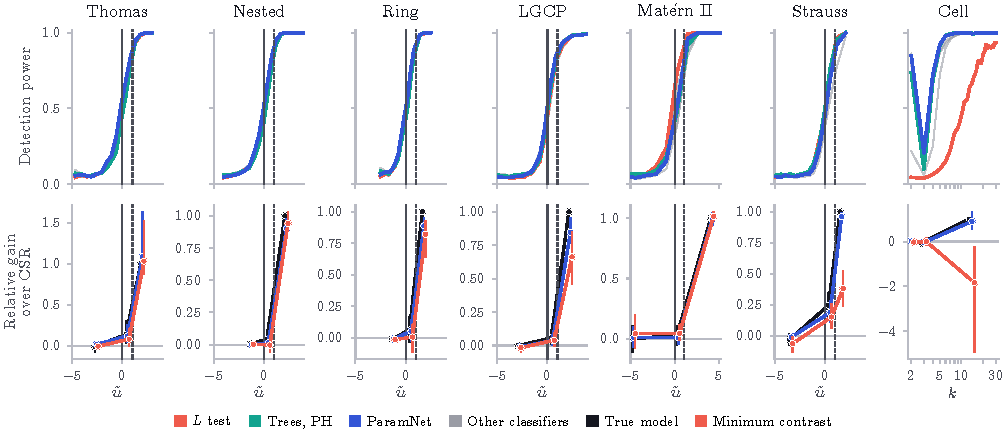
\includegraphics[width=\textwidth]{figs/v2/s_regime_detect}
\caption{Figure~\ref{fig:regime} per family, cell against $k$. Each family's coordinate $u=\log\eta+a\log\nb$ is
rescaled to $\tilde u=(u-u^\star_{0.5})/(u^\star_{0.9}-u^\star_{0.5})$, so that the $\tau=0.5$ boundary is at
$\tilde u=0$ (solid) and the $\tau=0.9$ boundary at $\tilde u=1$ (dashed). Top: detection power on the test
patterns of the $L$ test, trees on persistence summaries alone and ParamNet, and in grey every other classifier, all
tests of size $5\%$. Bottom: gain over CSR of the true model, ParamNet and minimum contrast on each stratum of the
evaluation set, as a share of the true model's gain in the family's strongest stratum (cell: $k\ge5$); $95\%$
bootstrap intervals over patterns. The $L$ test detects cell at its nominal $5\%$ for $k\le4$ and in $21\%$ of
patterns at $k=5$--$9$, where the learned detectors already detect almost all. Minimum contrast never selects cell,
and its fits to cell patterns at $k\ge5$ do worse than CSR.}
\label{fig:regime-detect}
\end{figure}

\begin{table*}[t]
\caption{The regime boundary per family; regime coordinates $\eta$ as in Table~\ref{tab:families}. Detection is a
test of size $5\%$; $u=\log\eta+a\log\nb$. AUC: detection predicted from $u$ alone and from all parameters (boosted
trees, out of fold). $u^\star(0.5)$: the boundary, where detection power reaches $0.5$, fitted on the reference
detector's out-of-fold training predictions, and recomputed on the test split for the $L$ test, for trees on
persistence summaries alone (``PH only'', which never sees $L$) and for ParamNet ($95\%$ bootstrap intervals over
$\theta$). Last column: share of each family's patterns in the structured regime. Higher AUC is better. The four
boundary estimates agree to within $0.25$ in $u$ in every family. Cell has no monotone coordinate. The $L$ test
detects it at its nominal $5\%$ for $k\le4$, while trees on the summary curves already detect $84\%$ of patterns at
$k=2$ (ParamNet $85\%$): the nearest-neighbour summaries see what $K$ cannot.}
\label{tab:regime}
\begin{center}
\footnotesize
\setlength{\tabcolsep}{4pt}
\begin{tabular}{@{}lrcrcccc@{}}
\toprule
& & AUC & \multicolumn{4}{c}{Boundary $u^\star(0.5)$} & In regime \\
\cmidrule(lr){4-7}
Family & $a$ & $u$ / all & Fitted & $L$ test & PH only & ParamNet & $\tau=0.5$ / $0.9$ \\
\midrule
Thomas      & $-0.30$ & $0.935$ / $0.940$ & $-1.77$ & $-1.71$ {\scriptsize[$-1.73$, $-1.68$]} & $-1.81$ {\scriptsize[$-1.88$, $-1.77$]} & $-1.71$ {\scriptsize[$-1.74$, $-1.61$]} & $0.39$ / $0.26$ \\
Nested      & $-0.35$ & $0.950$ / $0.959$ & $-1.95$ & $-1.95$ {\scriptsize[$-2.02$, $-1.92$]} & $-2.04$ {\scriptsize[$-2.09$, $-1.98$]} & $-1.95$ {\scriptsize[$-2.01$, $-1.86$]} & $0.58$ / $0.43$ \\
Ring        & $-0.36$ & $0.928$ / $0.945$ & $-1.70$ & $-1.82$ {\scriptsize[$-1.86$, $-1.77$]} & $-1.84$ {\scriptsize[$-1.89$, $-1.77$]} & $-1.65$ {\scriptsize[$-1.79$, $-1.65$]} & $0.50$ / $0.30$ \\
LGCP        & $-0.12$ & $0.927$ / $0.936$ & $+0.91$ & $+0.95$ {\scriptsize[$+0.92$, $+1.17$]} & $+0.91$ {\scriptsize[$+0.87$, $+1.00$]} & $+0.70$ {\scriptsize[$+0.69$, $+0.92$]} & $0.31$ / $0.21$ \\
Mat\'ern II & $-0.09$ & $0.957$ / $0.962$ & $-0.05$ & $-0.09$ {\scriptsize[$-0.10$, $-0.05$]} & $+0.01$ {\scriptsize[$-0.00$, $+0.06$]} & $+0.02$ {\scriptsize[$+0.00$, $+0.03$]} & $0.42$ / $0.37$ \\
Strauss     & $-0.11$ & $0.904$ / $0.914$ & $+0.14$ & $+0.18$ {\scriptsize[$+0.13$, $+0.22$]} & $+0.14$ {\scriptsize[$+0.13$, $+0.18$]} & $+0.16$ {\scriptsize[$+0.13$, $+0.22$]} & $0.21$ / $0.11$ \\
\bottomrule
\end{tabular}
\end{center}
\end{table*}

%==============================================================================
\section{ADDITIONAL RESULTS}
\label{app:results}

\subsection{Classification by Learner}
\label{app:classification}
\begin{itemize}
  \item Per-learner accuracy (Table~\ref{tab:classification}); confusion matrix (Figure~\ref{fig:confusion}).
\end{itemize}

\begin{table}[h]
\caption{Balanced accuracy over the eight families on the $192\,000$ test patterns. ``All'' is every pattern;
``$\tau{=}0.5$'' and ``$\tau{=}0.9$'' restrict to the structured regime at that detection power
(Section~\ref{sec:analysis}); ``Coarse'' is accuracy over the four mechanisms (CSR, clustered, regular, cell) at
$\tau{=}0.9$. Learners are named by input: ``classical'' is the summary curves, ``PH'' the persistence summaries of
the alpha and DTM$_{10}$ diagrams. Minimum contrast is penalized-contrast selection, which never selects Strauss or
cell. Intervals are within $\pm0.003$; higher is better throughout. Every learner meets the same limit on all
patterns, and ParamNet is ahead in the structured regime.}
\label{tab:classification}
\begin{center}
\footnotesize
% generated by paper/scripts -- do not edit; rerun python paper/scripts/make.py
\begin{tabular}{@{}lrrrr@{}}
\toprule
Classifier & All & $\tau{=}0.5$ & $\tau{=}0.9$ & Coarse \\
\midrule
Trees, classical + PH & 0.452 & 0.683 & 0.735 & 0.862 \\
ParamNet & 0.450 & 0.698 & 0.754 & 0.899 \\
Trees, classical & 0.447 & 0.675 & 0.726 & 0.858 \\
ParamNet, classical & 0.446 & 0.691 & 0.747 & 0.889 \\
Trees, PH & 0.436 & 0.665 & 0.719 & 0.849 \\
Logistic, classical & 0.396 & 0.583 & 0.620 & 0.783 \\
\midrule
Minimum contrast & 0.255 & 0.382 & 0.408 & 0.633 \\
\bottomrule
\end{tabular}

\end{center}
\end{table}

\begin{figure}[h]
\centering
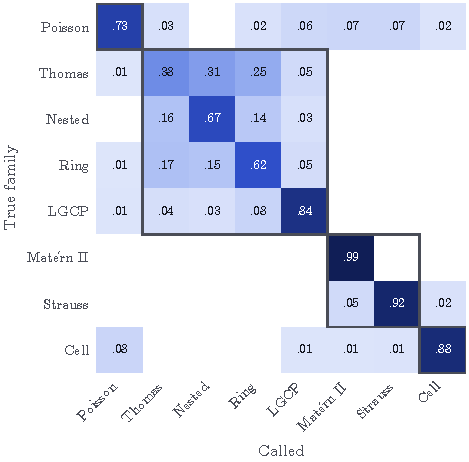
\includegraphics{figs/v2/f3_confusion}
\caption{Confusion matrix of ParamNet in the structured regime ($\tau=0.9$), rows normalized: the share of each true
family assigned to each family; blank cells are below $0.005$. Boxes: the mechanisms (CSR, clustered, regular, cell).
Confusions stay within the mechanism, mostly among Thomas, nested and ring, which produce the same patterns over part
of their parameter spaces.}
\label{fig:confusion}
\end{figure}

\subsection{Per-Family Fidelity}
\label{app:families-skill}
\begin{itemize}
  \item Per-family skill (Table~\ref{tab:families-skill}). (blocked: 5-seed rescoring)
\end{itemize}

\begin{table}[h]
\caption{Skill per family, $180$ patterns each ($179$ for ring). ``$\Delta$'' is ParamNet $-$ minimum contrast on the
same patterns, given the predicted and the true family, so minimum contrast's own skill is ParamNet's minus $\Delta$.
``$^\dagger$'' marks the families with no closed-form $K$: minimum contrast never selects them, and given the true
family it falls back to the training median. Skill can exceed $1$, because on a single replicate a fit can score
better than the true model. Intervals are $95\%$ bootstrap over patterns; higher skill and positive $\Delta$ favour
ParamNet.}
\label{tab:families-skill}
\begin{center}
\footnotesize
\setlength{\tabcolsep}{3.5pt}
% generated by paper/scripts -- do not edit; rerun python paper/scripts/make.py
\begin{tabular}{@{}lrrr@{}}
\toprule
Family & ParamNet & \begin{tabular}[b]{@{}r@{}}$\Delta$\\predicted\end{tabular} & \begin{tabular}[b]{@{}r@{}}$\Delta$\\true family\end{tabular} \\
\midrule
Thomas & \begin{tabular}[t]{@{}r@{}}$1.08$\\[-2pt]{\scriptsize[$0.90$, $1.60$]}\end{tabular} & \begin{tabular}[t]{@{}r@{}}$+0.10$\\[-2pt]{\scriptsize[$+0.01$, $+0.26$]}\end{tabular} & \begin{tabular}[t]{@{}r@{}}$+0.08$\\[-2pt]{\scriptsize[$+0.00$, $+0.21$]}\end{tabular} \\
Nested & \begin{tabular}[t]{@{}r@{}}$0.87$\\[-2pt]{\scriptsize[$0.79$, $0.94$]}\end{tabular} & \begin{tabular}[t]{@{}r@{}}$-0.03$\\[-2pt]{\scriptsize[$-0.12$, $+0.06$]}\end{tabular} & \begin{tabular}[t]{@{}r@{}}$+0.08$\\[-2pt]{\scriptsize[$-0.08$, $+0.34$]}\end{tabular} \\
Ring & \begin{tabular}[t]{@{}r@{}}$0.89$\\[-2pt]{\scriptsize[$0.82$, $0.96$]}\end{tabular} & \begin{tabular}[t]{@{}r@{}}$+0.11$\\[-2pt]{\scriptsize[$-0.01$, $+0.29$]}\end{tabular} & \begin{tabular}[t]{@{}r@{}}$+0.05$\\[-2pt]{\scriptsize[$-0.05$, $+0.18$]}\end{tabular} \\
LGCP & \begin{tabular}[t]{@{}r@{}}$0.83$\\[-2pt]{\scriptsize[$0.74$, $0.92$]}\end{tabular} & \begin{tabular}[t]{@{}r@{}}$+0.18$\\[-2pt]{\scriptsize[$-0.02$, $+0.38$]}\end{tabular} & \begin{tabular}[t]{@{}r@{}}$-0.05$\\[-2pt]{\scriptsize[$-0.14$, $+0.03$]}\end{tabular} \\
Mat\'ern II & \begin{tabular}[t]{@{}r@{}}$0.99$\\[-2pt]{\scriptsize[$0.87$, $1.12$]}\end{tabular} & \begin{tabular}[t]{@{}r@{}}$-0.09$\\[-2pt]{\scriptsize[$-0.25$, $+0.04$]}\end{tabular} & \begin{tabular}[t]{@{}r@{}}$-0.12$\\[-2pt]{\scriptsize[$-0.28$, $-0.01$]}\end{tabular} \\
\midrule
Strauss$^\dagger$ & \begin{tabular}[t]{@{}r@{}}$0.94$\\[-2pt]{\scriptsize[$0.87$, $1.00$]}\end{tabular} & \begin{tabular}[t]{@{}r@{}}$+0.55$\\[-2pt]{\scriptsize[$+0.40$, $+0.70$]}\end{tabular} & \begin{tabular}[t]{@{}r@{}}$+0.86$\\[-2pt]{\scriptsize[$+0.75$, $+0.97$]}\end{tabular} \\
Cell$^\dagger$ & \begin{tabular}[t]{@{}r@{}}$0.91$\\[-2pt]{\scriptsize[$0.50$, $1.34$]}\end{tabular} & \begin{tabular}[t]{@{}r@{}}$+2.81$\\[-2pt]{\scriptsize[$+1.13$, $+6.20$]}\end{tabular} & \begin{tabular}[t]{@{}r@{}}$+1.22$\\[-2pt]{\scriptsize[$+0.78$, $+2.14$]}\end{tabular} \\
\bottomrule
\end{tabular}

\end{center}
\end{table}

\subsection{Per-Family Estimation Error}
\label{app:estimation}
\begin{itemize}
  \item Table~\ref{tab:estimation}.
\end{itemize}

\begin{table}[h]
\caption{\new{Estimation error per family and estimator, given the true family. Cells are
$\mathrm{RMSE}(\log\theta)/\mathrm{s.d.}$ averaged over the family's targets, where $1$ is the error of predicting
the training mean. ``Val'' is the validation split; ``All'' is every test pattern; ``$\tau{=}0.5$'' and
``$\tau{=}0.9$'' restrict to the structured regime at that detection power. ``$\star$'' marks the lowest validation
error, the estimator a per-family selection rule would pick. Intervals are $95\%$ over test $\theta$; lower is
better. Every learner beats minimum contrast on every family.}}
\label{tab:estimation}
\begin{center}
\scriptsize
% generated by paper/scripts -- do not edit; rerun python paper/scripts/make.py
\begin{tabular}{@{}llrrrr@{}}
\toprule
Family & Estimator ($\star$ = best on val) & Val & All & $\tau{=}0.5$ & $\tau{=}0.9$ \\
\midrule
Thomas & \texttt{fusion\_curves\_alpha\_dtm10} $\star$ & 0.742 & 0.739 {\scriptsize [0.733, 0.746]} & 0.548 {\scriptsize [0.538, 0.558]} & 0.407 {\scriptsize [0.397, 0.417]} \\
Thomas & \texttt{fusion\_curves\_dtm10} & 0.743 & 0.741 {\scriptsize [0.734, 0.748]} & 0.559 {\scriptsize [0.549, 0.569]} & 0.426 {\scriptsize [0.416, 0.437]} \\
Thomas & \texttt{fusion\_curves\_alpha} & 0.745 & 0.741 {\scriptsize [0.735, 0.748]} & 0.556 {\scriptsize [0.546, 0.566]} & 0.427 {\scriptsize [0.416, 0.438]} \\
Thomas & \texttt{nn\_curves} & 0.746 & 0.741 {\scriptsize [0.735, 0.748]} & 0.553 {\scriptsize [0.543, 0.563]} & 0.415 {\scriptsize [0.404, 0.426]} \\
Thomas & \texttt{hgb\_classical\_ph} & 0.750 & 0.744 {\scriptsize [0.738, 0.750]} & 0.553 {\scriptsize [0.542, 0.563]} & 0.421 {\scriptsize [0.409, 0.430]} \\
Thomas & \texttt{hgb\_classical} & 0.752 & 0.745 {\scriptsize [0.739, 0.751]} & 0.555 {\scriptsize [0.545, 0.565]} & 0.425 {\scriptsize [0.414, 0.435]} \\
Thomas & min.\ contrast (tuned) & --- & 1.762 & --- & --- \\
Nested & \texttt{fusion\_curves\_alpha} & 0.729 & 0.717 {\scriptsize [0.711, 0.724]} & 0.638 {\scriptsize [0.631, 0.646]} & 0.570 {\scriptsize [0.564, 0.577]} \\
Nested & \texttt{fusion\_curves\_dtm10} $\star$ & 0.728 & 0.717 {\scriptsize [0.712, 0.725]} & 0.636 {\scriptsize [0.629, 0.644]} & 0.571 {\scriptsize [0.563, 0.578]} \\
Nested & \texttt{fusion\_curves\_alpha\_dtm10} & 0.729 & 0.719 {\scriptsize [0.714, 0.726]} & 0.639 {\scriptsize [0.631, 0.647]} & 0.571 {\scriptsize [0.564, 0.578]} \\
Nested & \texttt{nn\_curves} & 0.731 & 0.719 {\scriptsize [0.714, 0.726]} & 0.642 {\scriptsize [0.635, 0.649]} & 0.576 {\scriptsize [0.569, 0.583]} \\
Nested & \texttt{hgb\_classical\_ph} & 0.735 & 0.724 {\scriptsize [0.719, 0.731]} & 0.641 {\scriptsize [0.634, 0.649]} & 0.573 {\scriptsize [0.565, 0.580]} \\
Nested & \texttt{hgb\_classical} & 0.740 & 0.726 {\scriptsize [0.721, 0.733]} & 0.647 {\scriptsize [0.641, 0.655]} & 0.580 {\scriptsize [0.572, 0.587]} \\
Nested & min.\ contrast (tuned) & --- & 2.250 & --- & --- \\
LGCP & \texttt{hgb\_classical} & 0.542 & 0.541 {\scriptsize [0.536, 0.545]} & 0.356 {\scriptsize [0.348, 0.365]} & 0.279 {\scriptsize [0.269, 0.289]} \\
LGCP & \texttt{fusion\_curves\_alpha\_dtm10} $\star$ & 0.540 & 0.541 {\scriptsize [0.536, 0.546]} & 0.364 {\scriptsize [0.355, 0.372]} & 0.289 {\scriptsize [0.280, 0.299]} \\
LGCP & \texttt{nn\_curves} & 0.542 & 0.541 {\scriptsize [0.536, 0.546]} & 0.366 {\scriptsize [0.357, 0.374]} & 0.301 {\scriptsize [0.290, 0.311]} \\
LGCP & \texttt{hgb\_classical\_ph} & 0.543 & 0.541 {\scriptsize [0.537, 0.546]} & 0.359 {\scriptsize [0.350, 0.367]} & 0.283 {\scriptsize [0.273, 0.293]} \\
LGCP & \texttt{fusion\_curves\_alpha} & 0.541 & 0.541 {\scriptsize [0.537, 0.546]} & 0.365 {\scriptsize [0.356, 0.373]} & 0.293 {\scriptsize [0.283, 0.303]} \\
LGCP & \texttt{fusion\_curves\_dtm10} & 0.544 & 0.542 {\scriptsize [0.537, 0.547]} & 0.363 {\scriptsize [0.354, 0.371]} & 0.295 {\scriptsize [0.284, 0.306]} \\
LGCP & min.\ contrast (tuned) & --- & 0.873 & --- & --- \\
Mat\'ern II & \texttt{fusion\_curves\_alpha} & 0.238 & 0.233 {\scriptsize [0.230, 0.236]} & 0.114 {\scriptsize [0.111, 0.117]} & 0.089 {\scriptsize [0.087, 0.092]} \\
Mat\'ern II & \texttt{nn\_curves} & 0.240 & 0.233 {\scriptsize [0.230, 0.236]} & 0.103 {\scriptsize [0.101, 0.105]} & 0.084 {\scriptsize [0.082, 0.086]} \\
Mat\'ern II & \texttt{hgb\_classical\_ph} $\star$ & 0.238 & 0.234 {\scriptsize [0.231, 0.237]} & 0.109 {\scriptsize [0.106, 0.112]} & 0.088 {\scriptsize [0.086, 0.090]} \\
Mat\'ern II & \texttt{hgb\_classical} & 0.240 & 0.235 {\scriptsize [0.232, 0.238]} & 0.110 {\scriptsize [0.108, 0.113]} & 0.089 {\scriptsize [0.086, 0.092]} \\
Mat\'ern II & \texttt{fusion\_curves\_alpha\_dtm10} & 0.241 & 0.236 {\scriptsize [0.233, 0.239]} & 0.116 {\scriptsize [0.113, 0.119]} & 0.090 {\scriptsize [0.088, 0.093]} \\
Mat\'ern II & \texttt{fusion\_curves\_dtm10} & 0.245 & 0.243 {\scriptsize [0.240, 0.246]} & 0.137 {\scriptsize [0.134, 0.140]} & 0.118 {\scriptsize [0.116, 0.121]} \\
Mat\'ern II & min.\ contrast (tuned) & --- & 0.315 & --- & --- \\
Ring & \texttt{fusion\_curves\_dtm10} & 0.706 & 0.709 {\scriptsize [0.702, 0.716]} & 0.601 {\scriptsize [0.591, 0.611]} & 0.457 {\scriptsize [0.448, 0.466]} \\
Ring & \texttt{fusion\_curves\_alpha} $\star$ & 0.703 & 0.709 {\scriptsize [0.702, 0.716]} & 0.599 {\scriptsize [0.590, 0.607]} & 0.449 {\scriptsize [0.439, 0.459]} \\
Ring & \texttt{fusion\_curves\_alpha\_dtm10} & 0.705 & 0.710 {\scriptsize [0.703, 0.717]} & 0.599 {\scriptsize [0.590, 0.608]} & 0.461 {\scriptsize [0.451, 0.470]} \\
Ring & \texttt{hgb\_classical\_ph} & 0.705 & 0.710 {\scriptsize [0.703, 0.717]} & 0.590 {\scriptsize [0.581, 0.600]} & 0.436 {\scriptsize [0.428, 0.445]} \\
Ring & \texttt{nn\_curves} & 0.707 & 0.711 {\scriptsize [0.704, 0.718]} & 0.605 {\scriptsize [0.596, 0.614]} & 0.457 {\scriptsize [0.449, 0.466]} \\
Ring & \texttt{hgb\_classical} & 0.715 & 0.715 {\scriptsize [0.708, 0.722]} & 0.604 {\scriptsize [0.595, 0.613]} & 0.462 {\scriptsize [0.453, 0.471]} \\
Ring & min.\ contrast (tuned) & --- & 1.475 & --- & --- \\
Cell & \texttt{hgb\_classical\_ph} $\star$ & 0.132 & 0.137 {\scriptsize [0.135, 0.140]} & 0.137 {\scriptsize [0.135, 0.140]} & 0.137 {\scriptsize [0.135, 0.140]} \\
Cell & \texttt{fusion\_curves\_dtm10} & 0.137 & 0.141 {\scriptsize [0.139, 0.143]} & 0.141 {\scriptsize [0.139, 0.143]} & 0.141 {\scriptsize [0.139, 0.143]} \\
Cell & \texttt{fusion\_curves\_alpha\_dtm10} & 0.138 & 0.143 {\scriptsize [0.140, 0.145]} & 0.143 {\scriptsize [0.140, 0.145]} & 0.143 {\scriptsize [0.140, 0.145]} \\
Cell & \texttt{fusion\_curves\_alpha} & 0.148 & 0.153 {\scriptsize [0.151, 0.156]} & 0.153 {\scriptsize [0.151, 0.156]} & 0.153 {\scriptsize [0.151, 0.156]} \\
Cell & \texttt{hgb\_classical} & 0.154 & 0.159 {\scriptsize [0.157, 0.161]} & 0.159 {\scriptsize [0.157, 0.161]} & 0.159 {\scriptsize [0.157, 0.161]} \\
Cell & \texttt{nn\_curves} & 0.172 & 0.173 {\scriptsize [0.171, 0.176]} & 0.173 {\scriptsize [0.171, 0.176]} & 0.173 {\scriptsize [0.171, 0.176]} \\
Cell & min.\ contrast (tuned) & --- & 0.547 & --- & --- \\
Strauss & \texttt{hgb\_classical} $\star$ & 0.534 & 0.546 {\scriptsize [0.537, 0.552]} & 0.203 {\scriptsize [0.197, 0.212]} & 0.102 {\scriptsize [0.097, 0.108]} \\
Strauss & \texttt{hgb\_classical\_ph} & 0.538 & 0.546 {\scriptsize [0.538, 0.552]} & 0.203 {\scriptsize [0.195, 0.211]} & 0.099 {\scriptsize [0.095, 0.105]} \\
Strauss & \texttt{fusion\_curves\_alpha} & 0.543 & 0.555 {\scriptsize [0.547, 0.561]} & 0.226 {\scriptsize [0.218, 0.234]} & 0.110 {\scriptsize [0.104, 0.115]} \\
Strauss & \texttt{nn\_curves} & 0.544 & 0.555 {\scriptsize [0.547, 0.561]} & 0.262 {\scriptsize [0.255, 0.270]} & 0.152 {\scriptsize [0.146, 0.157]} \\
Strauss & \texttt{fusion\_curves\_alpha\_dtm10} & 0.552 & 0.562 {\scriptsize [0.555, 0.568]} & 0.225 {\scriptsize [0.218, 0.234]} & 0.113 {\scriptsize [0.106, 0.119]} \\
Strauss & \texttt{fusion\_curves\_dtm10} & 0.556 & 0.565 {\scriptsize [0.558, 0.571]} & 0.251 {\scriptsize [0.243, 0.258]} & 0.137 {\scriptsize [0.131, 0.142]} \\
Strauss & min.\ contrast (tuned) & --- & 0.664 & --- & --- \\
\bottomrule
\end{tabular}

\end{center}
\end{table}

\subsection{Persistent Homology by Filtration}
\label{app:filtrations}
\begin{itemize}
  \item Filtration contrast (Table~\ref{tab:filtrations}).
  \item 40-input ablation only if it lands, as one heatmap; otherwise remove the promise.
\end{itemize}

\begin{table}[h]
\caption{Which filtration carries what topology adds. Columns are the same network, trainer and stopping rule on four
input sets: ``both'' persistence filtrations (ParamNet), ``alpha'' or ``DTM'' alone, and ``neither'' (the summary
curves only). Cells are $\mathrm{RMSE}(\log\theta)/\mathrm{s.d.}$ in the structured regime ($\tau{=}0.9$), where $1$
is the error of predicting the training mean, then balanced accuracy at $\tau{=}0.9$, then ParamNet's end-to-end skill
minus each column's, paired on the same $1\,439$ patterns. Intervals are $95\%$ over test $\theta$ (errors, accuracy)
or over patterns (skill). One training seed, so differences under about $0.005$ in error are within seed noise.}
\label{tab:filtrations}
\begin{center}
\footnotesize
% generated by paper/scripts -- do not edit; rerun python paper/scripts/make.py
\begin{tabular}{@{}lrrrr@{}}
\toprule
 & both & alpha & DTM & neither \\
\midrule
Thomas & 0.407 {\scriptsize [0.397, 0.417]} & 0.427 {\scriptsize [0.416, 0.438]} & 0.426 {\scriptsize [0.416, 0.437]} & 0.415 {\scriptsize [0.404, 0.426]} \\
Nested & 0.571 {\scriptsize [0.564, 0.578]} & 0.570 {\scriptsize [0.564, 0.577]} & 0.571 {\scriptsize [0.563, 0.578]} & 0.576 {\scriptsize [0.569, 0.583]} \\
LGCP & 0.289 {\scriptsize [0.280, 0.299]} & 0.293 {\scriptsize [0.283, 0.303]} & 0.295 {\scriptsize [0.284, 0.306]} & 0.301 {\scriptsize [0.290, 0.311]} \\
Mat\'ern II & 0.090 {\scriptsize [0.088, 0.093]} & 0.089 {\scriptsize [0.087, 0.092]} & 0.118 {\scriptsize [0.116, 0.121]} & 0.084 {\scriptsize [0.082, 0.086]} \\
Ring & 0.461 {\scriptsize [0.451, 0.470]} & 0.449 {\scriptsize [0.439, 0.459]} & 0.457 {\scriptsize [0.448, 0.466]} & 0.457 {\scriptsize [0.449, 0.466]} \\
Cell & 0.143 {\scriptsize [0.140, 0.145]} & 0.153 {\scriptsize [0.151, 0.156]} & 0.141 {\scriptsize [0.139, 0.143]} & 0.173 {\scriptsize [0.171, 0.176]} \\
Strauss & 0.113 {\scriptsize [0.106, 0.119]} & 0.110 {\scriptsize [0.104, 0.115]} & 0.137 {\scriptsize [0.131, 0.142]} & 0.152 {\scriptsize [0.146, 0.157]} \\
\midrule
accuracy, $\tau$=0.9 & 0.754 {\scriptsize [0.752, 0.759]} & 0.749 {\scriptsize [0.746, 0.753]} & 0.746 {\scriptsize [0.742, 0.750]} & 0.747 {\scriptsize [0.744, 0.750]} \\
skill, both $-$ column & --- & -0.016 {\scriptsize [-0.055, +0.019]} & -0.003 {\scriptsize [-0.048, +0.046]} & +0.011 {\scriptsize [-0.033, +0.053]} \\
\bottomrule
\end{tabular}

\end{center}
\end{table}

\subsection{Other}
\begin{itemize}
  \item Gallery of observed patterns vs fits: random draws per family, including wrong-family fits.
  \item Mat\'ern~I out-of-library result only if Limitations cites it; otherwise cut.
\end{itemize}


\end{document}
